\section{The Indicator (haylij) and Governor (kadhkhudah)}
\begin{mdframed}[backgroundcolor=cyan!5, rightmargin=1em, leftmargin=1em]
This  book is a bit of a nightmare to understand, the basic rules are jumbled in with definitions, delineations, and interpolated text across two chapters. In reading them I've often referred to Dykes \textsl{Carmen Astrologicum} and \textsl{Persian Nativities Vol. II} as well as Holden's \textsl{Abu'Ali Al-Khayyat: The Judgment of Nativities}, Hand's \textsl{Omar of Tiberias: Three Books on Nativities}, Deb Houldings Notes on Book III, Valens and Robert Zoller's DMA Course. As a result, the text in this section of the book has been extensively re-organized; an effort has been made to include references to the original chapter and line numbers.
\end{mdframed}

\subsection{Definitions}
Dorotheus describes some of the conditions that effect the ability of a planet to be effective (strong) or ineffective (weak):
\begin{description}[style=multiline,leftmargin=7em]
\item[Eastern]\mn{1.4}a planet at least 15°\footnote{The 15° is a generalized value; Dorotheus gives 18° for \Mars, 19° for \Mercury\, and the same is usually assumed (see Dykes) for \Venus. Essentially, you want the planet to be visible, so the distance from the \Sun\, can vary depending on whether the planet is \textsl{superior} (\Saturn, \Jupiter, \Mars) or \textsl{inferior} (\Venus,\Mercury) and also based on the birth latitude. It is sometimes necessary to check actual \href{https://www.sunrise-and-sunset.com/en/sun}{sunrise-sunset times} for the day in question.} from the \Sun\, and rising ahead of it
\item[Western ]\mn{1.5}a planet at least 15° from the \Sun\, and setting after it
\item[Station] stationing direct or retrograde within 7 days before or after birth
\item[USB]\mn{1.6} a planet less than 15° from the \Sun\, is ``under the \Sun's'' rays or beams (usually referenced as USB); it is essentially invisible
\end{description}

Planets that are direct, eastern, and visible\footnote{see appendix \ref{appendix:visibility}:Visibility} are better able to effect what they signify.

\subsection{Possible Indicator}
Find the indicator (hyleg) first; begin with the \Sun\, in a day chart, the \Moon\, in a night chart \textsl{unless} the \Moon\, \mn{1.10} is New, Full, or making a phase, in which case she will be the indicator.

Once the indicator is identified, by default, its term lord (if it qualifies), becomes the governor (alcocoden).

\subsubsection{The Lights}
If\mn{1.24} either light is in its own domicile (\Sun\, in \Leo, \Moon\, in \Cancer) and its term lord is in square or trine that light becomes the indicator and its term lord the governor\footnote{Presumably if this is true for both lights you would need to use the sect light or the best positioned light or possibly, the light whose term lord had the closest aspect.}

\subsubsection{The Sun}
In a day chart, the \Sun\, is the default indicator unless it is found to be in one of the following situations:
\vspace{-0.5em}
\begin{itemize}[topsep=0em,itemsep=0em]
\item \mn{1.15}in the 8th or 7th in a feminine sign, look to the \Moon
\item \mn{1.21}if cadent, look to the \Moon\, and if it is also cadent, look to the Ascendant
\end{itemize}

\subparagraph{An Exception}
If \mn{1.25} the \Sun\, is in the first degrees \textsl{[0 thru 9?]} of \Aries\, and its term or domicile lord aspects it, that planet becomes the indicator and, presumably, his term lord the governor.

\subsubsection{The Moon}
\vspace{-0.5em}
In a day chart, if the \Sun\, does not qualify as the indicator, the \Moon\, will if she is found in one of the following situations:
\begin{itemize}[topsep=0em,itemsep=0em]
\item \mn{1.17}in the 10th or 11th in a feminine sign
\item \mn{1.18}in the 7th or 8th regardless of sign
\item if the \Moon\, is in the 12th or 9th, regardless of sign, \mn{1.21}look to the Ascendant\footnote{The preceding definitions imply that the \Moon\, must be above the horizon in a day chart and not cadent. As the \Sun\, has already been disqualified we are to move on to examining the Ascendant.}
\end{itemize}

In a night chart, the \Moon\, is the default indicator unless it is found to be in one of the following situations:
\begin{itemize}[topsep=0em,itemsep=0em]
\item \mn{1.19, 20}the \Moon\, is cadent or its term lord is USB, in which case the \Sun\, is the indicator if it is in the 4th or 5th, \mn{1.21}otherwise look to the Ascendant
\end{itemize}

\subsubsection{The Ascendant}
If the \Sun\, or \Moon\, have been disqualified from being the indicator, or their term lords have been disqualified from being the governor, examine the Ascendant degree. If its term lord is disqualified, examine the Ascendant's domicile lord and \mn{1.12} if it is USB \textsl{[or cadent?]}, examine its lord \textsl{[term lord?]}\footnote{Dorotheus then tells us to see if the place \textsl{[sign?]} of this lord is masculine or feminine but he does not say if one or the other disqualifies the lord.}

\vspace{-0.5em}
\subsection{Term Lord (Governor)}
If the term lord of the indicator is found to be in one of the following situations  it is disqualified, move on to the next possible indicator.

\begin{itemize}[topsep=0em, itemsep=0em]
\item \mn{1.18, 19} USB
\item \mn{1.11} cadent
\end{itemize}

\subsection{Indications}
\subsubsection{From the Sun}



\subsubsection{From the Moon}
If \mn{1.7} the \Moon\, on the third day after the birth is in the term of:

\begin{itemize}[topsep=0em,itemsep=0em]
\item a benefic which is in a good place trine the \Moon\, while the \Moon\, is in an angular or succedent place ``then say that all of the nativity's condition is good''

\item either \mn{1.9} a benefic or malefic in a good place aspecting the \Moon, ``then it will be mediocre''

\item a \mn{1.8} malefic which is in an angle while Fortune is opposite the \Moon\, ``then say [that there is] no doubt that the nativity is bad''
\end{itemize}

\subsubsection{The Ascendant}
If \mn{1.22,23} the lord \textsl{[term or domicile? it's not clear]} of the Ascendant is disqualified from being governor ``then say [that there is] ruination in this nativity and that he [the native] will have no upbringing'' unless there is a benefic in the ascendant sign within 15° of the Ascendant.

\subsection{Example Chart 3.1.1 Circumambulation}
\vspace{0.5em}
\begin{mdframed}[backgroundcolor=cyan!5, rightmargin=1em, leftmargin=1em]
This particular chart is dated to February 26, 381 CE JC according to Ben Dykes (CAD p17) and so could not possibly have been included in Dorotheus' original manuscript as he lived in the 1st century, not the 4th. The other nine charts in the text have been dated between 12 and 44 CE. Dykes also believes the chart is based on the sidereal zodiac, although the oblique ascensions given agree to the tropical tables for the period.
\end{mdframed}

\vspace{-1em}
\begin{figure}[H]
\centering
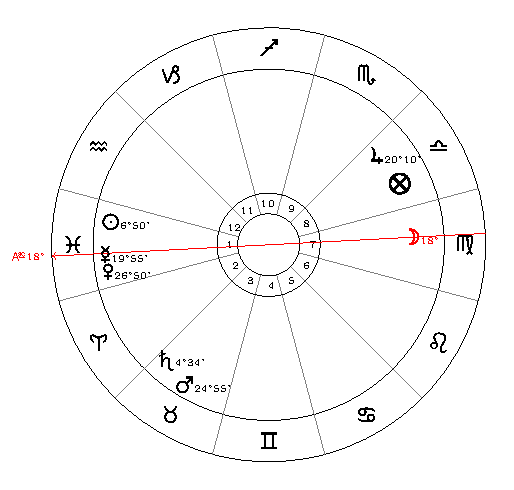
\includegraphics[width=0.8\textwidth]{charts/3_1_01}
\vspace{-1em}
\caption{Chart 01: A Man}
\end{figure}

Figure 3.1 is the chart of a person ``born in the ninety-sixth year of the years of Darinus [Diocletian] in the month of Mihr on the second day in one and a half equinoctial hours of daylight\footnote{The \Moon\, is missing from the chart in the text, assuming the Ascendant and \Sun\, degrees are roughly accurate, it should be around 18-19 \Virgo.}....in the 4th clime''. The author uses the chart to ``explain...the length of life and the number of years as \textsl{[he attempts]} [to compute it].''

\begin{quote}
\textsl{``I \mn{1.29} wanted to know the places of the haylaj among which he was born because they are five places, and none of the planets was in them except in the ascendant in which the \Sun\, was; and it is the best of places.''}
\end{quote}

The author has not spelled out ``the five places'' at this point, at a guess he is referring to the 1st, 7th, 11th, 10th, and 9th(?).  He says he chooses the 1st because the \Sun\, is there; that it is above the horizon and so cadent by degree does not appear to matter, it is angular by whole sign rules. He then begins to direct the Ascendant (not the \Sun\, or its term lord) through the bounds.

\begin{quote}
\textsl{``I \mn{1.34-5}wanted to know in how many years the ascendant would conjoin with the rays of \Mars. I took the eighteen degrees of the ascendent and I found in the [tables for] my clime and the twelve parts [signs] [that] placed under it [was] three hundred and fifty-two [time] degrees and thirty seconds''}
\end{quote}

The Ascendant is at 18 \Pisces\, and \Mars\, is at 24 Taurus\, 55, sending its sextile (\Sextile) ray to 24\Pisces 55. The author wants to know how long it will take for the degree imprinted by \Mars\, sextile ray to rise up, by primary (diurnal) motion, to the Ascendant degree. He uses a technique commonly called \textsl{circumambulation} that relies on the use of ``tables'', in this example, those for the 4th clime, to find the corresponding oblique ascension degrees for 18 \Pisces\, and 24 \Taurus\, 55. The 4th clime corresponds to Rhodes with a latitude of 36N\footnote{See \href{https://journals.sagepub.com/doi/10.1177/002182869302400105}{Verification of Parallax in Ptolemy's Hand Tables} by José Chabás and Anne Tihon }.

\begin{quote}
\textsl{``Then \mn{1.36-7} I took the twenty-four degrees and fifty minutes where \Mars\, cast its rays to \Pisces\, and I found the rising-times under this [to be] three hundred and fifty-six [time] degrees and forty-eight minutes''}
\end{quote}

Dykes gives the date of the chart as 381 CE, using \href{https://horoscopes.astro-seek.com/calculate-ascensional-rising-times/?latitude=100&narozeni_lat_custom_stupne=36&narozeni_lat_custom_minuty=0&narozeni_lat_custom_smer=0&narozeni_rok=381&aya=&oa=4&decimal=1}{Astro-Seek's Online Calculator} to calculate the oblique ascensions for custom latitude 36N in the year 381 CE the values for the two longitudes are within a few minutes of those given in the text:

\begin{quote}
\textsl{ ``[S]o I subtracted the three hundred and fifty-two [degrees] and thirty [minutes] which belong to the ascendent, and there were left four [time] degrees and eighteen minutes. And I said that the degrees of the ascendent would conjoin with the sextile rays of \Mars\, in four years and a fifth and a tenth of a year.''}
\end{quote}
From the Astro-seek tables (see Figure 3.2):
\begin{itemize}[topsep=0em,itemsep=0em]
\item[] \texttt{18\Pisces\,        352°28'    vs       352°30'}
\item[] \texttt{24\Pisces\,        356°52'    vs       356°48'}
\end{itemize}

\begin{figure}[H]
\centering
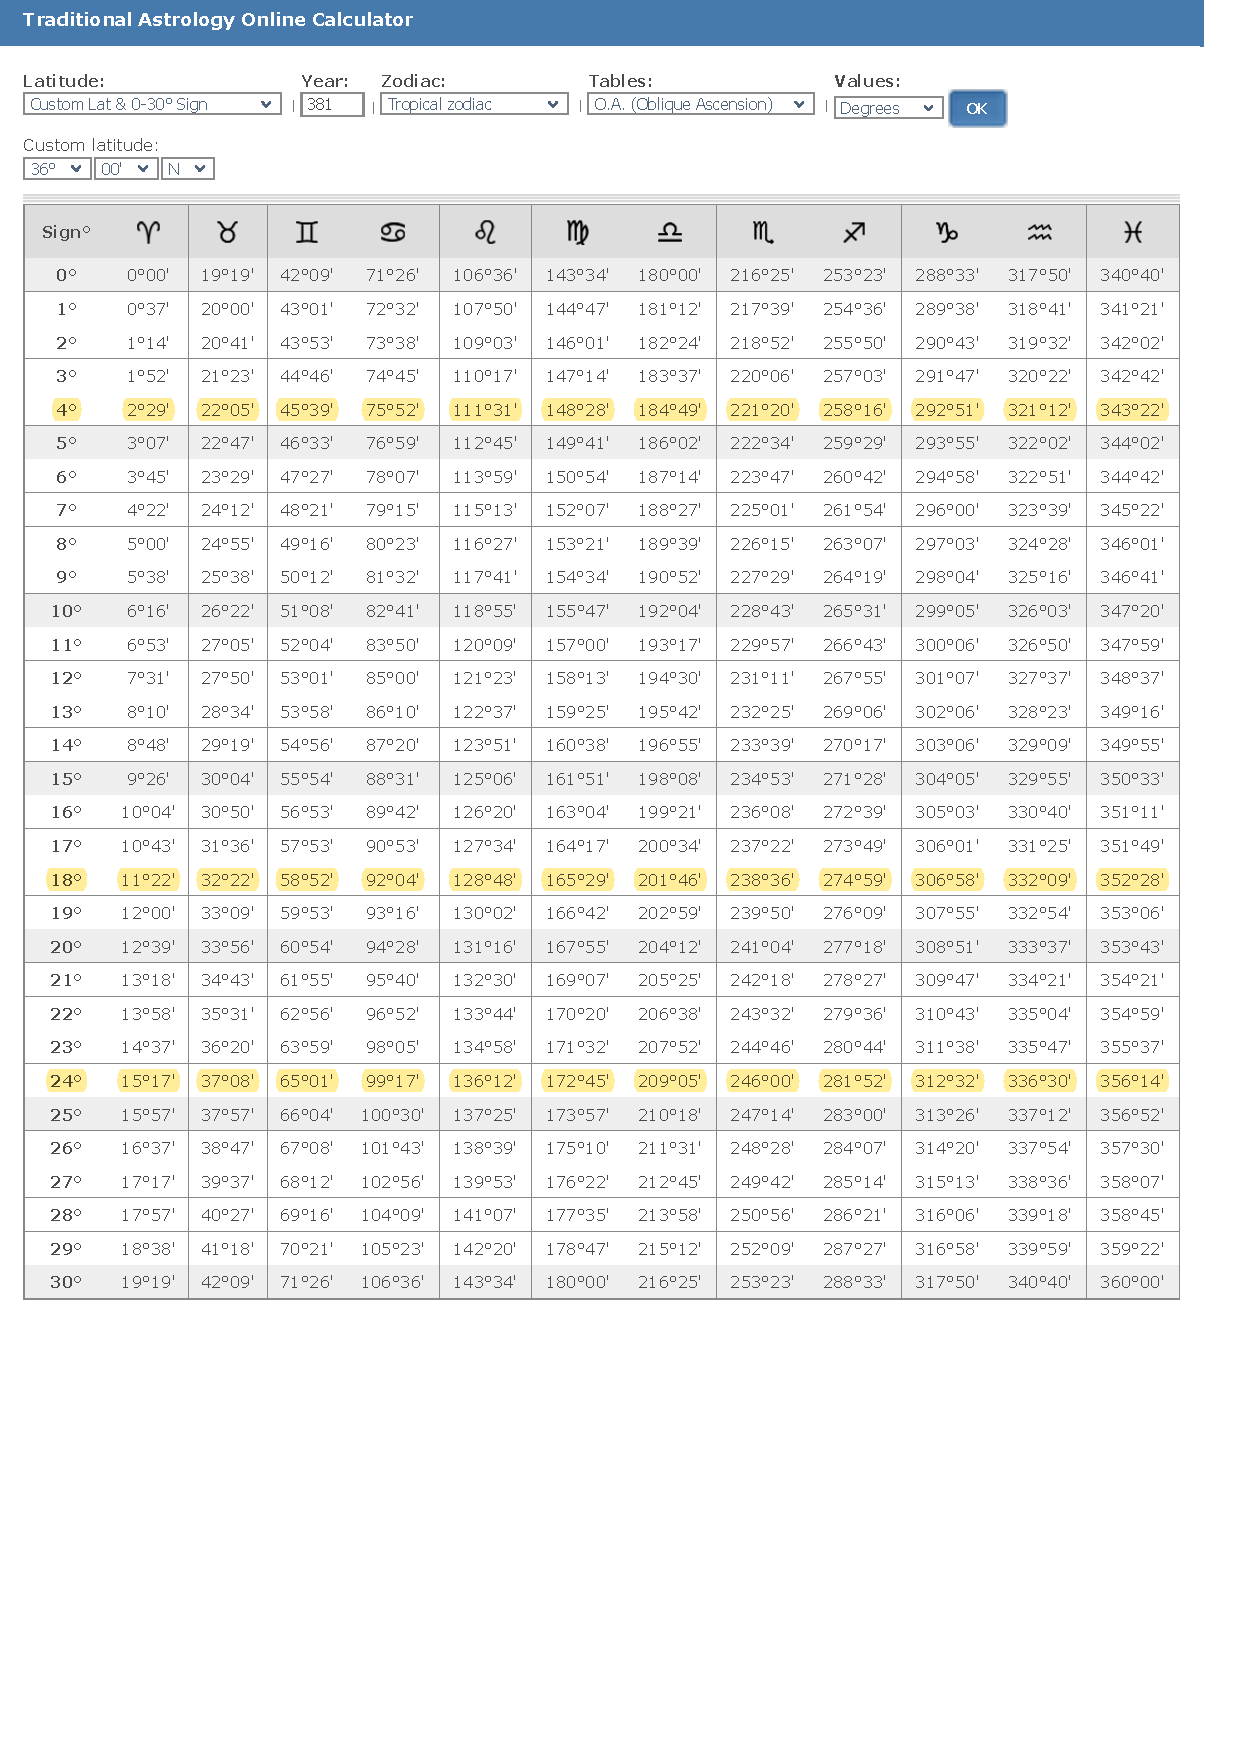
\includegraphics[width=0.9\textwidth]
	{diagrams/3.1.1-OA-Table }
\vspace{-8em}
\caption{OA table for Chart 3.1.1 calculated on Astro-seek}
\end{figure}

The difference between 352°30' and 356°48' is 4°18' or 4 years, 3 months (18/60 = 0.3 x 12 = 3.6) and 18 (.6 x 30) days\footnote{Dykes explains the author's calculation as 18/60 = .3, 1/5 = .2 and 1/10 = .1 so 4 year plus 1/5 and 1/10 of a year (p.184 fn 34). It computes to the same 4 years + 365 x (1/5 + 1/10) = 4 years + 365 x 3/10 = 4 years 109.5 days or 4 years, 3 months, 18 days}.

\begin{quote}
\textsl{``Because \mn{1.38} \Venus\, [is] in this term, it dissolves the fear and misery that \Mars\, indicates and he will not die, but this misery will pass by him because whenever the rays of the benefics are found with the rays of the malefics, then the benefic dissolves whatever the malefic indicates; but if the malefic and its term cast rays without the benefics, then it will not be long before he dies.''}
\end{quote}

The sextile of \Mars\, falls at 24 \Pisces\, 55 in the terms of \Mars\, which run from 19° to 27° \Pisces. \Venus\, is sitting at 25 \Pisces\, 50 so she is in the same terms as the sextile ray and therefore removes its malice.

Next the author looked at when the Ascendant would contact 4 \Taurus\, 34, the degree the body of \Saturn\, was projecting itself to at the time of the birth. Using the same set of tables for the 4th clime, the oblique ascension of 4 \Taurus\, 34 was found to be 22° 21' (the Astro-seek table yields 22°23.8' if interpolation is used between 4 \Taurus\, and 5 \Taurus). Taking the difference between the Ascendant's OA of 352°30' and \Saturn's OA of 22°21' leaves 29°51' equating to 29 years, 1/2 + 1/4 + 1/10th of a year or 29 years 10 months and 10 days, the age at which the Ascendant will conjoin with \Saturn's degree.

\begin{quote}
\textsl{``Because \mn{1.50} the \Sun\, cast its rays from sextile to the first term of \Taurus\, were \Saturn\, was staying, the heat of the \Sun\, will drive away all the maleficence of \Saturn, and the harsh misery will pass him by, and he will not die.''}
\end{quote}

The first terms of \Taurus\, run from 0° to 7°. \Saturn\, projects to 4 \Taurus\, and the \Sun, at 6\Pisces, throws his sextile to 6 \Taurus\, so both \Saturn\, and the \Sun's ray fall in the same set of terms. The \Sun\, is apparently acting as a benefic here.